\documentclass[tikz,border=2pt]{standalone}
\usepackage{amsmath,amssymb}
\usepackage{tikz}
\usetikzlibrary{arrows.meta}

\begin{document}
% A probability function assigns a number in [0,1] to every event: P(empty) = 0, P(S) = 1,
% and disjoint events add. Here S = {1,...,6} with a fair die.
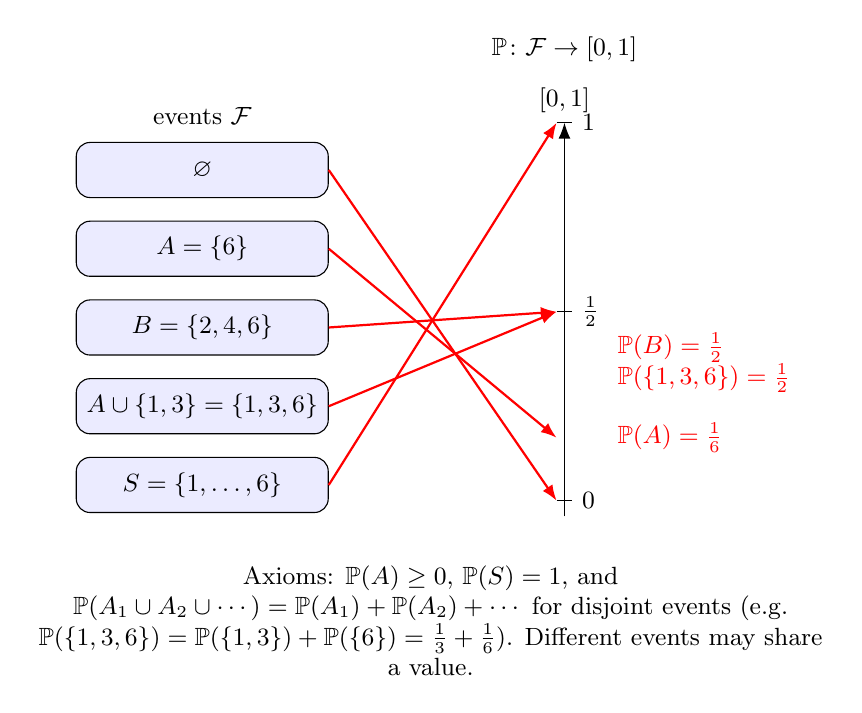
\begin{tikzpicture}[every node/.style={font=\small}, >={Latex[length=2mm]}]
	\node[draw, rounded corners=5pt, fill=blue!8, minimum width=3.2cm, minimum height=0.7cm] (e0) at (0,3.0) {$\varnothing$};
	\node[draw, rounded corners=5pt, fill=blue!8, minimum width=3.2cm, minimum height=0.7cm] (e1) at (0,2.0) {$A=\{6\}$};
	\node[draw, rounded corners=5pt, fill=blue!8, minimum width=3.2cm, minimum height=0.7cm] (e2) at (0,1.0) {$B=\{2,4,6\}$};
	\node[draw, rounded corners=5pt, fill=blue!8, minimum width=3.2cm, minimum height=0.7cm] (e3) at (0,0) {$A\cup\{1,3\}=\{1,3,6\}$};
	\node[draw, rounded corners=5pt, fill=blue!8, minimum width=3.2cm, minimum height=0.7cm] (e4) at (0,-1.0) {$S=\{1,\dots,6\}$};
	\node[anchor=south] at (0,3.45) {events $\mathcal{F}$};
	\draw[->] (4.6,-1.4) -- (4.6,3.6) node[above] {$[0,1]$};
	\draw (4.5,-1.2) -- (4.7,-1.2) node[right] {$0$};
	\draw (4.5,1.2) -- (4.7,1.2) node[right] {$\tfrac12$};
	\draw (4.5,3.6) -- (4.7,3.6) node[right] {$1$};
	\draw[->, red, thick] (e0.east) -- (4.5,-1.2);
	\draw[->, red, thick] (e1.east) -- (4.5,-0.4);
	\draw[->, red, thick] (e2.east) -- (4.5,1.2);
	\draw[->, red, thick] (e3.east) -- (4.5,1.2);
	\draw[->, red, thick] (e4.east) -- (4.5,3.6);
	\node[red, anchor=west] at (5.15,-0.4) {$\mathbb{P}(A)=\tfrac16$};
	\node[red, anchor=west, align=left] at (5.15,0.55) {$\mathbb{P}(B)=\tfrac12$\\ $\mathbb{P}(\{1,3,6\})=\tfrac12$};
	\node[anchor=south] at (4.6,4.25) {$\mathbb{P}\colon\mathcal{F}\to[0,1]$};
	\node[anchor=north, align=flush center, text width=10cm] at (2.9,-1.9) {Axioms: $\mathbb{P}(A)\ge0$, $\mathbb{P}(S)=1$, and $\mathbb{P}(A_1\cup A_2\cup\cdots)=\mathbb{P}(A_1)+\mathbb{P}(A_2)+\cdots$ for disjoint events (e.g. $\mathbb{P}(\{1,3,6\})=\mathbb{P}(\{1,3\})+\mathbb{P}(\{6\})=\tfrac13+\tfrac16$). Different events may share a value.};
\end{tikzpicture}
\end{document}
